\documentclass[11pt, a4paper]{article}

% --- ESSENTIAL PACKAGES ---

% Font Encoding and Input
\usepackage[T1]{fontenc} % Use 8-bit T1 fonts to ensure proper character rendering
\usepackage[utf8]{inputenc} % Allows direct use of UTF-8 characters (e.g., é, ö, à)
\usepackage{amsmath} % For \text{} in math mode

% Page Layout and Margins
\usepackage{geometry}
\geometry{
    a4paper,
    left=2.5cm,
    right=2.5cm,
    top=3cm,
    bottom=3cm
}

% Professional Fonts (Latin Modern)
\usepackage{lmodern}
\usepackage{helvet} % For Helvetica font, used for the main title

% --- COLOR AND STYLING ---

% Color Management
\usepackage[dvipsnames]{xcolor} % Use dvipsnames for a wider range of predefined colors

% Define a professional color palette
\definecolor{primary}{HTML}{0A369D}  % A deep, professional blue
\definecolor{secondary}{HTML}{4472CA} % A lighter, complementary blue
\definecolor{darkgray}{HTML}{333333}  % For body text, better than pure black
\definecolor{customgreen}{HTML}{5E8B7E} % A muted green for accents
\definecolor{titleblue}{HTML}{082A75} % A darker, rich blue for the main title

\color{darkgray} % Set the default text color

% Section and Title Styling
\usepackage{titlesec}
\titleformat{\section}
  {\normalfont\Large\bfseries\color{primary}} % Format for the section title
  {\thesection}{1em}{} % Section number, spacing, and the title itself
\titleformat{\subsection}
  {\normalfont\large\bfseries\color{secondary}}
  {\thesubsection}{1em}{}
\titleformat{\subsubsection}
  {\normalfont\bfseries\color{customgreen}}
  {\thesubsubsection}{1em}{}

% --- IMAGES AND GRAPHICS ---

% Standard package for including images
\usepackage{graphicx}
\graphicspath{{images/}} % Optional: specify a folder for your images
\usepackage{float} % Improved control over figure placement with [H] option

% --- LISTS AND ENUMERATIONS ---

% Customize list environments
\usepackage{enumitem}
% The 'textcolor' option sets the color for the item's text
\setlist[itemize,1]{label=\textcolor{primary}{\textbullet}, textcolor=primary} 
\setlist[itemize,2]{label=\textcolor{secondary}{\textendash}, textcolor=secondary}

% --- HYPERLINKS ---

% Hyperlink styling for URLs and cross-references
\usepackage{hyperref}
\hypersetup{
    colorlinks=true,
    linkcolor=primary,
    filecolor=magenta,      
    urlcolor=secondary,
    citecolor=customgreen,
    pdftitle={My Professional Document},
    pdfpagemode=FullScreen,
}

% --- TYPOGRAPHY AND MICRO-ADJUSTMENTS ---

% Improves the justification and spacing of text for a cleaner look
\usepackage{microtype}

% --- DOCUMENT CONTENT EXAMPLE ---

% For placeholder text
\usepackage{lipsum} 

\title{A Biologically-Grounded Generative Framework for Modeling Prostate Cancer Progression}
\author{}
\date{}

\begin{document}

\maketitle

\section{Introduction}
Prostate cancer (PCa) represents a paramount public health challenge, ranking as the second most common cancer in men worldwide \cite{CaraccioloCastello2024,DulleaOSullivan2025}. In 2020 alone, over 1.4 million new cases were diagnosed globally, and it stands as the fifth leading cause of cancer-related death among men, responsible for approximately 375,000 deaths that year \cite{CereserEvangelista2023,GammelSolari2024,DharCendejasGomez2024}. The epidemiological trajectory is alarming, with projections indicating that the number of cases will more than double to 2.9 million by 2040, driven largely by an aging global population \cite{UdovicichJia2025,SungFerlay2021}.

The management of PCa is fraught with complexity, stemming from the dual risks of overdiagnosis and undertreatment. Widespread screening with prostate-specific antigen (PSA) has led to the frequent detection of indolent, clinically insignificant cancers, resulting in overtreatment and significant morbidity \cite{PadhaniSchoots2023,JenaTaneja2018,CaraccioloCastello2022}. Curative therapies, such as radical prostatectomy (RP) or radiation therapy (RT), carry risks of urinary incontinence and erectile dysfunction that impact quality of life \cite{GeboersMeijer2023,GiorgioRapa2024}. Conversely, many PCa deaths are due to the late diagnosis of aggressive or metastatic disease \cite{PadhaniSchoots2023}.

This diagnostic dilemma is exacerbated by the limitations of conventional tools. Standard imaging modalities like CT and bone scintigraphy (BS) have suboptimal accuracy for staging, often failing to detect small-volume metastases \cite{EsenSeymen2023,GiovacchiniPicchio2014,LingJong2021}. The stakes of such misstaging are incredibly high; the distinction between localized and metastatic disease carries profound prognostic implications, with the 5-year survival rate dropping from nearly 100\% to as low as 30-40\% \cite{WangODwyer2024,CereserEvangelista2023}. The high rate of biochemical recurrence (BCR) following curative-intent therapy underscores the urgent need for more sensitive and specific methods for staging, risk stratification, and treatment planning \cite{JinCai2024,CombesPalma2022}.

This confluence of high incidence, significant mortality, and the profound challenges in diagnosis and management establishes a clear and pressing need for a new generation of predictive models. While artificial intelligence has shown promise, current systems often struggle to provide generalizable solutions that can effectively take into account all available multimodal data. A significant gap remains between current implementations and the robust, reliable tools required for routine clinical practice. Therefore, new models must be capable of integrating the full spectrum of clinical data to provide a more accurate, personalized, and holistic understanding of each patient's disease trajectory. This work aims to lay the groundwork for such a paradigm.

\section{Aims}
The primary aim of this work is to lay the groundwork for a new generation of predictive models in prostate cancer by addressing the fundamental challenges of data heterogeneity and model interpretability. The core objectives are twofold:
\begin{itemize}
    \item To propose a framework for creating a standardized, longitudinal, and multimodal dataset that captures the complete patient journey.
\end{itemize}

%https://g.co/gemini/share/abe1a144d8a5
\begin{figure}[H]
\centering
 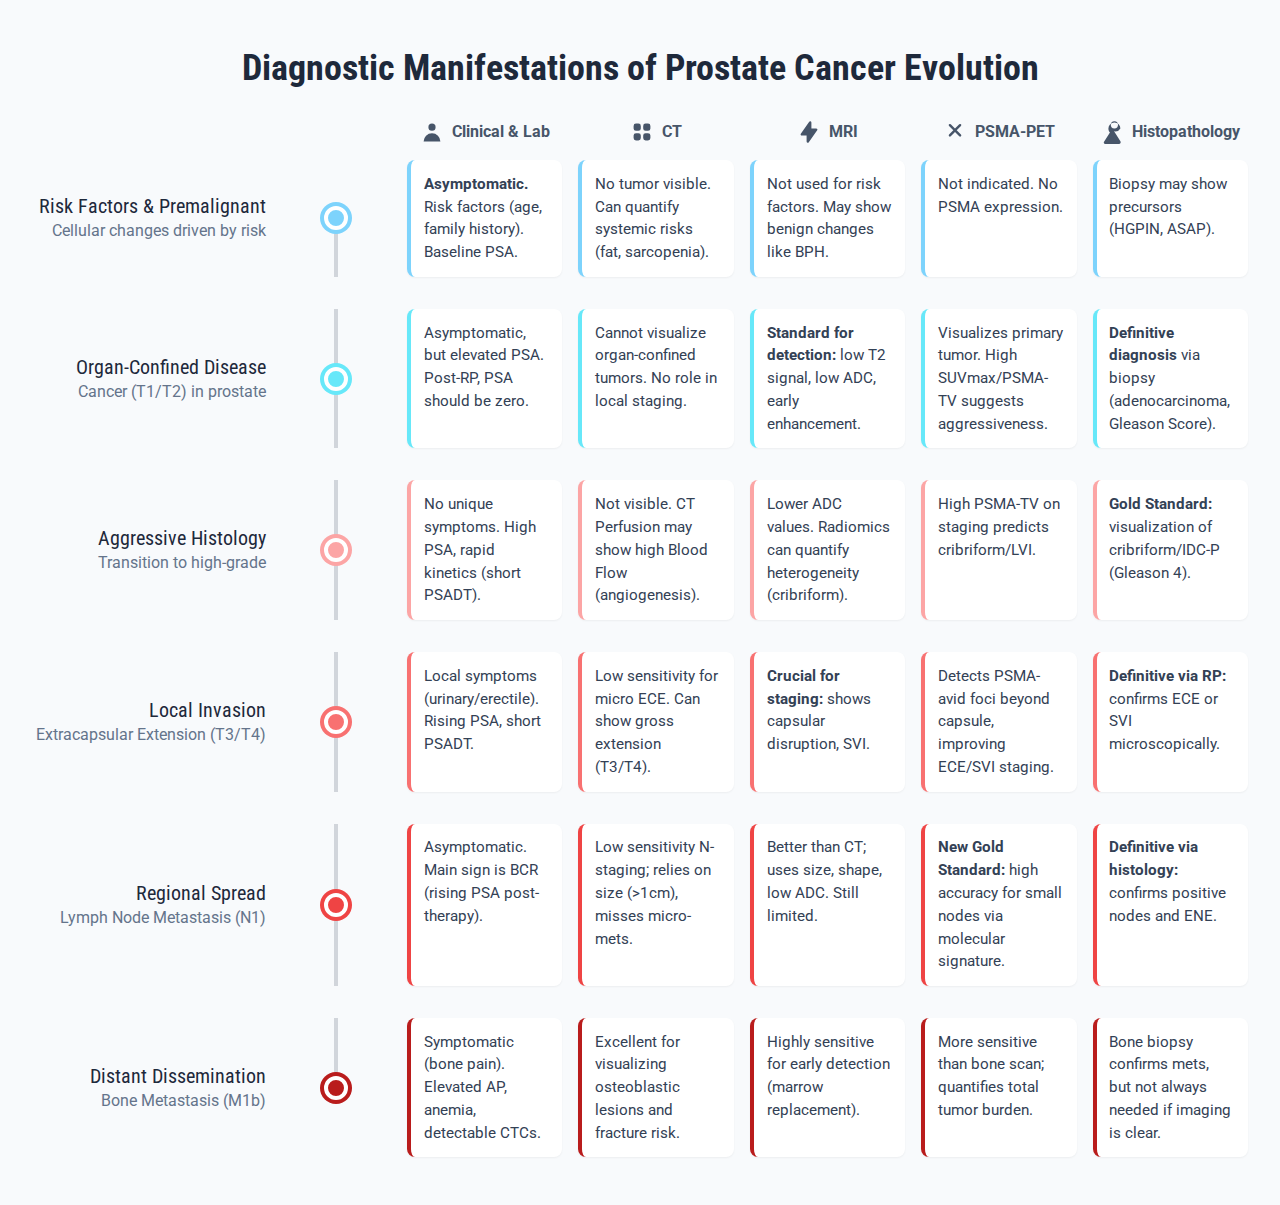
\includegraphics[width=\textwidth]{pe.png}
 \caption{An infographic illustrating the natural history of prostate cancer.}
\label{fig:prostate_evolution}
\end{figure}

\begin{itemize}
    
    \item To conceptualize a disentangled generative model that leverages this high-quality data. Crucially, this model will be designed to incorporate strong inductive biases based on domain knowledge, specifically the two interacting axes of disease progression: the TNM-based pathophysiological evolution of the cancer and the dynamic, patient-specific host characteristics. By doing so, the model will be better equipped to handle the complexities of incomplete, multimodal, and temporally evolving clinical data.
\end{itemize}
A secondary, yet significant, aim is to reduce the clinical burden of documentation. We envision a system where the model's disentangled latent representations, which correspond to meaningful clinical and biological concepts, can be used to automatically generate structured, accurate, and consistent clinical reports, thereby freeing up valuable physician time.



\section{The Evolution and Pathophysiology of Prostate Cancer}
The natural history of prostate cancer (PCa) is a multi-step process that begins with cellular changes and can culminate in a lethal, metastatic disease. This evolution involves the acquisition of specific biological capabilities that allow cancer cells to grow locally, invade surrounding tissues, and disseminate to distant organs \cite{OrzechowskaAnusewicz2022}. The progression is not always linear and can be significantly altered by therapeutic interventions.

\subsection{Premalignant State and Risk Factors}
The development of PCa is initiated by cellular changes within the prostate's internal environment, which can become more prone to cancer development through processes like inflammation and reduced oxygen (hypoxia) \cite{BianchiFriasDamodarasamy2019, MartinCaraballo2024}. These initial changes happen within the prostate gland, usually in an area called the peripheral zone (PZ), where precancerous conditions like high-grade prostatic intraepithelial neoplasia (H-PIN) can form \cite{UnknownAuthor2017}. The specific drivers for these changes, such as age, genetics, and lifestyle, are patient-specific factors discussed in a later section.

\subsection{Organ-Confined Disease (Early Cancer)}
This stage marks the formation of a true tumor that is still contained entirely within the prostate gland, corresponding to TNM stages T1 and T2 \cite{PasoglouMichoux2016, UnknownAuthor2017}. Here, cancerous cells form a distinct mass, which may be too small to be felt or seen on imaging (T1) or may be large enough to be felt during a rectal exam (T2) \cite{CaglicKovac2019, OliveiraFerreira2023}. If the cancer is low-grade (Gleason Score 6 or less), its cells are still relatively well-organized and have almost no potential to spread, making it suitable for active surveillance \cite{UnknownAuthor2017, DrostOsses2019}. Tumor growth at this stage is fueled by male hormones (androgens) that activate the androgen receptor (AR) \cite{UnknownAuthor2014, MartinCaraballo2024}. The prostate's outer layer, the capsule, acts as a natural barrier, keeping the cancer contained.

\subsection{Acquisition of Aggressive Histological Features (High-Risk Features)}
A pivotal moment in the cancer's evolution is when it becomes more disorganized and aggressive. This is identified by a pathologist who sees specific high-risk patterns under the microscope. The most important of these are the cribriform pattern and/or Intraductal Carcinoma of the Prostate (IDC-P) \cite{GordetskySchaffer2022, HesterbergGordetsky2021, BernardinoSayyid2023}. The appearance of these disorganized, fused cell structures is a strong warning sign that the cancer has a much higher chance of invading locally, spreading to distant sites, and returning after treatment \cite{HesterbergGordetsky2021, GaoZhang2020}.

\subsection{Local Invasion Beyond the Prostate (Extracapsular Extension)}
This stage marks the tumor's transition from organ-confined to locally advanced (T3/T4), a critical turning point with a worse prognosis \cite{OliveiraFerreira2023, CarpagnanoEusebi2020}. To escape the prostate, the cancer cells must break through the gland's capsule. They do this by altering the local environment, producing enzymes that dissolve the surrounding tissue matrix and interacting with specialized cells called fibroblasts that help pave the way for invasion \cite{UnknownAuthor2012, PenetKakkad2017}. Once outside the capsule, the cancer can spread into the surrounding fat (ECE; pT3a) or invade nearby structures like the seminal vesicles (SVI; pT3b), both of which dramatically increase the risk of recurrence and death \cite{FanXie2022, ErbayOzden2020}. Anatomically, this breach is significant because it gives the cancer direct access to the rich network of blood vessels and lymphatic channels around the prostate, opening the door for it to travel throughout the body \cite{FanXie2022}.

\subsection{Regional Spread to Pelvic Lymph Nodes (Lymph Node Metastasis)}
After breaking out of the prostate, cancer cells can travel through the lymphatic system to nearby lymph nodes in the pelvis. This process confirms the disease has become systemic, meaning it has the ability to spread throughout the body, which significantly reduces the chances of a cure with local treatments like surgery or radiation alone \cite{CaglicBarrett2018, ZarzourGalgano2017}. The cancer typically follows predictable anatomical routes to the pelvic lymph nodes (obturator, iliac, and presacral nodes), which is classified as N1 disease. If the cancer spreads to lymph nodes beyond the pelvis, it is considered distant metastatic disease (M1a) and carries a worse prognosis \cite{CaglicBarrett2018, OliveiraFerreira2023}.

\subsection{Distant Dissemination to Bone (Bone Metastasis)}
The final and most dangerous stage of progression is the spread of cancer to distant sites, most commonly the bones. Prostate cancer has a unique affinity for the bone environment, a concept known as the "seed and soil" theory, where circulating cancer cells ("seed") find the bone ("soil") to be a fertile ground to grow \cite{RucciAngelucci2014, PawanRich2024}. Anatomically, the cancer often spreads to the axial skeleton (spine, pelvis) through a network of veins called Batson's plexus, leading to severe pain, fractures, and a poor prognosis \cite{UnknownAuthor2012, RucciAngelucci2014, MohseniniaZamaniSiahkali2024}.

\subsection{The Impact of Treatment on Disease Evolution}
Therapeutic interventions fundamentally alter this natural history.
\begin{itemize}
    \item \textbf{Radical Prostatectomy:} For localized disease, RP can be curative by removing the primary tumor, which provides definitive pathological staging and can significantly reduce mortality risk compared to observation \cite{LuoYi2019, HerlemannCowan2024, LeyhBannurahDellOglio2019}.
    \item \textbf{Hormonal Therapy:} For advanced disease, Androgen Deprivation Therapy (ADT) targets the AR signaling axis by lowering testosterone, initially causing tumor regression \cite{MartinCaraballo2024, UnknownAuthor2014, BellmuntKheoh2016}. However, this pressure selects for castration-resistant PCa (CRPC), where cancer cells develop mechanisms to bypass the hormonal blockade, what may lead to a more aggressive, lethal disease state \cite{MartinCaraballo2024, UnknownAuthor2014}.
    \item \textbf{Radioligand Therapy (RLT):} For advanced mCRPC, $\text{[}^{177}\text{Lu]}\text{Lu-PSMA-617}$ RLT provides a targeted approach that delivers radiation directly to PSMA-positive cancer cells. This has been shown to significantly prolong survival and delay disease progression in heavily pre-treated patients, thereby altering the terminal course of the disease \cite{FizaziHerrmann2023, Keam2022}.
\end{itemize}

\section{Diagnostic Manifestations of Prostate Cancer Evolution}
Each stage of PCa's pathophysiological evolution produces a unique signature of findings across various diagnostic modalities. These modalities provide complementary views of the same underlying biological state.

\subsection{Histopathology}
Histopathology provides the definitive diagnosis and is the gold standard against which all other modalities are measured. At the \textbf{Premalignant} stage, biopsy may reveal precursor lesions like H-PIN \cite{UnknownAuthor2017}. For \textbf{Early Cancer}, it diagnoses acinar adenocarcinoma and establishes the Gleason Score (GS) \cite{UnknownAuthor2014, TruongFrye2018}. The acquisition of \textbf{High-Risk Features} is diagnosed by the direct visualization of cribriform architecture or IDC-P, which are graded as Gleason Pattern 4 \cite{GordetskySchaffer2022}. For \textbf{Extracapsular Extension}, the pathologist microscopically confirms tumor cells beyond the capsule (ECE) or in the seminal vesicles (SVI) \cite{OliveiraFerreira2023}. Pelvic lymph node dissection allows for the definitive confirmation of \textbf{Lymph Node Metastasis}, including the number of involved nodes and the presence of extranodal extension (ENE) \cite{CaglicBarrett2018}. Finally, a bone biopsy can confirm \textbf{Bone Metastasis}, though it is less commonly performed if the clinical context is clear \cite{GoodeWang2023}.

\subsection{Magnetic Resonance Imaging (MRI)}
mpMRI is the standard for non-invasively assessing the local extent of PCa. In \textbf{Early Cancer}, it detects tumors as T2-hypointense lesions with restricted diffusion (low ADC) and early contrast enhancement, reflecting high cellularity and vascularity \cite{CarpagnanoEusebi2020, KurhanewiczSwanson2002}. It can infer \textbf{High-Risk Features} through quantitative metrics; progressively lower ADC values and more pronounced metabolic shifts on MRSI (low citrate, high choline) correlate with higher Gleason grades \cite{DuenwegBobholz2023, KurhanewiczSwanson2002}. MRI excels at staging \textbf{Extracapsular Extension} by identifying anatomical signs like capsular disruption or SVI. The Length of Capsular Contact (LCC) is a quantifiable metric for predicting microscopic ECE \cite{PriesterMota2024, CaglicKovac2019}. While MRI can detect suspicious lymph nodes based on size and low ADC, its accuracy is limited for small \textbf{Lymph Node Metastasis} \cite{CaglicKovac2019}. For \textbf{Bone Metastasis}, MRI is highly sensitive, visualizing the replacement of fatty bone marrow by tumor cells often before structural changes are visible on other modalities \cite{DammeTombal2021}. Post-treatment changes are also visible; effective ADT, for example, causes a significant reduction in citrate on MRSI, reflecting metabolic atrophy of the cancer cells \cite{KurhanewiczSwanson2002}.

\subsection{Computed Tomography (CT)}
Conventional CT plays a limited role in early-stage disease but is crucial for assessing advanced disease. It cannot directly visualize microscopic \textbf{High-Risk Features}, but functional techniques like CT Perfusion can detect the associated increase in angiogenesis (high BF and BV) \cite{HuellnerPauli2014}. CT has low sensitivity for subtle \textbf{Extracapsular Extension} but can depict gross invasion of adjacent structures \cite{OliveiraFerreira2023}. For \textbf{Lymph Node Metastasis}, CT is a standard tool but is limited by its reliance on nodal size \cite{ZarzourGalgano2017}. Its primary strength is in evaluating \textbf{Bone Metastasis}, where it excels at visualizing the characteristic dense, osteoblastic lesions and assessing fracture risk \cite{HayakawaTabata2020}.

\subsection{PSMA-PET Imaging}
PSMA-PET provides a whole-body molecular snapshot of the disease. It visualizes \textbf{Early Cancer} and can infer \textbf{High-Risk Features}, as the intensity of PSMA uptake ($SUV_{max}$) and tumor volume (PSMA-TV) correlate strongly with Gleason grade and the presence of cribriform histology \cite{ZouJiao2020, VetroneMei2023}. Due to its high sensitivity, it is superior to conventional imaging for detecting \textbf{Extracapsular Extension} and has become the new gold standard for non-invasively staging \textbf{Lymph Node Metastasis}, accurately identifying small, metastatic nodes missed by CT and MRI \cite{VetroneMei2023, SiegelMiller2018}. It also detects \textbf{Bone Metastasis} with higher sensitivity than bone scans, visualizing viable tumor cells and allowing for precise quantification of the total skeletal tumor burden, a powerful predictor of survival \cite{KleiburgGeusOei2025}. PSMA-PET is also valuable for monitoring treatment. Post-therapy Lutetium-177 scintigraphy (SPECT/CT) allows for direct visualization of treatment delivery and patient-specific dosimetry \cite{HennrichEder2022, PathmanandavelCrumbaker2022}. However, ADT can modulate PSMA expression, sometimes causing a transient 'PSMA flare' that can mimic disease progression \cite{AmalachandranSivathapandi2024, MohseniniaZamaniSiahkali2024}.

\section{Patient Characteristics Influencing PCa Biology and Prognosis}
The natural history and response to treatment in prostate cancer are not solely dictated by the tumor's biological stage but are significantly modulated by a host of patient-specific factors. These characteristics influence risk, disease aggressiveness, and the effectiveness of therapeutic interventions.

\subsection{Inherent Risk Factors and Patient History}
The most established non-modifiable risk factors for PCa are age, and genetic predisposition/family history \cite{UnknownAuthor2017, PerezCornagoDunneram2021}.
\begin{itemize}
    \item \textbf{Age:} Ageing is the most widely recognized risk factor for PCa \cite{UnknownAuthor2017, KaderBrangsch2021}. The incidence significantly increases after age 40, with peak rates between 65 and 75 years \cite{BianchiFriasDamodarasamy2019, UnknownAuthor2017}. The aged prostate microenvironment promotes PCa development through elevated macrophage infiltration, extracellular matrix remodeling, and increased tissue hypoxia \cite{BianchiFriasDamodarasamy2019, MartinCaraballo2024}. Early-onset PCa (diagnosed before age 55) is often considered a distinct clinical-pathological phenotype with a potentially poorer prognosis \cite{OrzechowskaAnusewicz2022, MilonasVenclovas2017}.
    \item \textbf{Family History and Genetics:} A positive family history is a well-established risk factor, with a two- to threefold increased risk for men with an affected first-degree relative \cite{CarpagnanoEusebi2020, UnknownAuthor2017}. Inherited genes like \textit{BRCA2} can cause more aggressive cancers and are associated with earlier onset and worse prognosis \cite{UnknownAuthor2017, CarpagnanoEusebi2020, JiHuang2017, ChenWang2023}.
\end{itemize}

\subsection{Signs, Symptoms, and Laboratory Findings}
During the \textbf{Risk Factors} and \textbf{Early Cancer} stages, patients are typically asymptomatic, and diagnosis relies on PSA screening \cite{PasoglouMichoux2016}. Advanced PSA derivatives like the PHI or 4K Score can improve specificity for higher-grade disease \cite{ChenWang2023}. The development of \textbf{High-Risk Features} often correlates with a higher PSA level or more rapid PSA kinetics (short PSADT) \cite{HesterbergGordetsky2021, Tisman2013}. The onset of local urinary or erectile symptoms (dysuria, hematuria, weak flow) often signals \textbf{Extracapsular Extension} \cite{PasoglouMichoux2016, BalzsAntal2021, HeZhong2024}. \textbf{Lymph Node Metastasis} is usually clinically silent, with its primary sign being biochemical recurrence (a rising PSA) after local therapy \cite{CaglicBarrett2018}. The stage of \textbf{Bone Metastasis} is frequently symptomatic, with bone pain being the most common complaint \cite{UnknownAuthor2014}. Laboratory findings become critical at this stage, with elevated serum Alkaline Phosphatase (AP), bone turnover markers (BTMs), and anemia reflecting the systemic impact of skeletal disease \cite{GoodeWang2023, UnknownAuthor2014}. Following ADT, the clinical picture changes, and prognosis is heavily reliant on PSA kinetics, where a low PSA nadir and a long time to reach it signal a better outcome \cite{BellmuntKheoh2016, OKAHATANO2024, HuMao2023}.

\subsection{Body Composition, Performance Status, and Comorbidities}
A patient's general health, body composition, and functional status significantly impact prognosis and treatment tolerance.
\begin{itemize}
    \item \textbf{Body Composition (Adiposity and Sarcopenia):} Lifestyle choices leading to obesity promote inflammation and hormonal shifts that can fuel cancer growth \cite{UnknownAuthor2017, DickermanTorfadottir2019}. CT can quantify adverse body composition features like high visceral fat or sarcopenia, which are linked to worse outcomes \cite{LeePark2020, GrecoPiccolo2024}. Greater visceral fat is associated with a higher risk of advanced and fatal PCa \cite{WilsonTaaffe2022, DickermanTorfadottir2019}. Conversely, sarcopenia (low muscle mass) is associated with an increased risk of mortality and poor tolerance to chemotherapy \cite{LopezNewton2021, PablosRodrguezPinoSedeo2022}. Treatment side effects, such as ADT-induced sarcopenia and fat gain, also become important prognostic factors \cite{PablosRodrguezPinoSedeo2022, CariolouChristakoudi2024}.
    \item \textbf{Performance Status (ECOG/Karnofsky):} The functional status of a patient (e.g., Karnofsky Performance Status) is a critical prognostic indicator, especially in advanced PCa, and is included in multiple nomograms to predict survival \cite{UnknownAuthor2014}.
    \item \textbf{Comorbidities:} Overall health status and comorbidities, particularly cardiovascular disease (CVD), significantly influence treatment selection and overall survival \cite{HerlemannCowan2024, CooperbergBroering2009}. ADT is associated with an increased risk of cardiovascular mortality \cite{HubanksBoorjian2014, UnknownAuthor2017}.
\end{itemize}

\subsection{Bridging Diagnostics and Pathophysiology: The Challenge of Intersecting Axes}
The comprehensive evaluation of prostate cancer requires a multi-modal synthesis of information that acknowledges two critical, intersecting axes: the tumor's intrinsic biological evolution (approximated by TNM staging) and the unique characteristics of the patient host. As detailed, the underlying biological processes—from cellular disorganization in \textbf{High-Risk Features} to the systemic impact of \textbf{Bone Metastasis}—manifest as a complex mosaic of findings across histopathology, laboratory studies, and advanced imaging. Each modality offers a unique window into the disease: MRI excels at local soft tissue anatomy, PSMA-PET reveals whole-body molecular activity, CT defines bone structure and body composition, and lab markers track the systemic burden.

However, a significant clinical challenge is that information from both axes is often incomplete and collected at different time points. For instance, definitive histopathology is often only available after surgery, while patient characteristics like body composition or performance status change over time, especially in response to treatment. The interplay between the tumor's state and the patient's state is dynamic and complex. Consequently, there is a critical need to infer the complete, time-resolved state of the disease by integrating all available data with a deep understanding of the known pathophysiological pathways. This inferential process is essential for accurate diagnosis, prognosis, and treatment planning, and highlights the potential for advanced computational models, including generative AI, to help fill these informational gaps and create a truly personalized model of each patient's cancer journey.


%https://gemini.google.com/app/d582944f26c12f98
\begin{figure}[H]
    \centering
    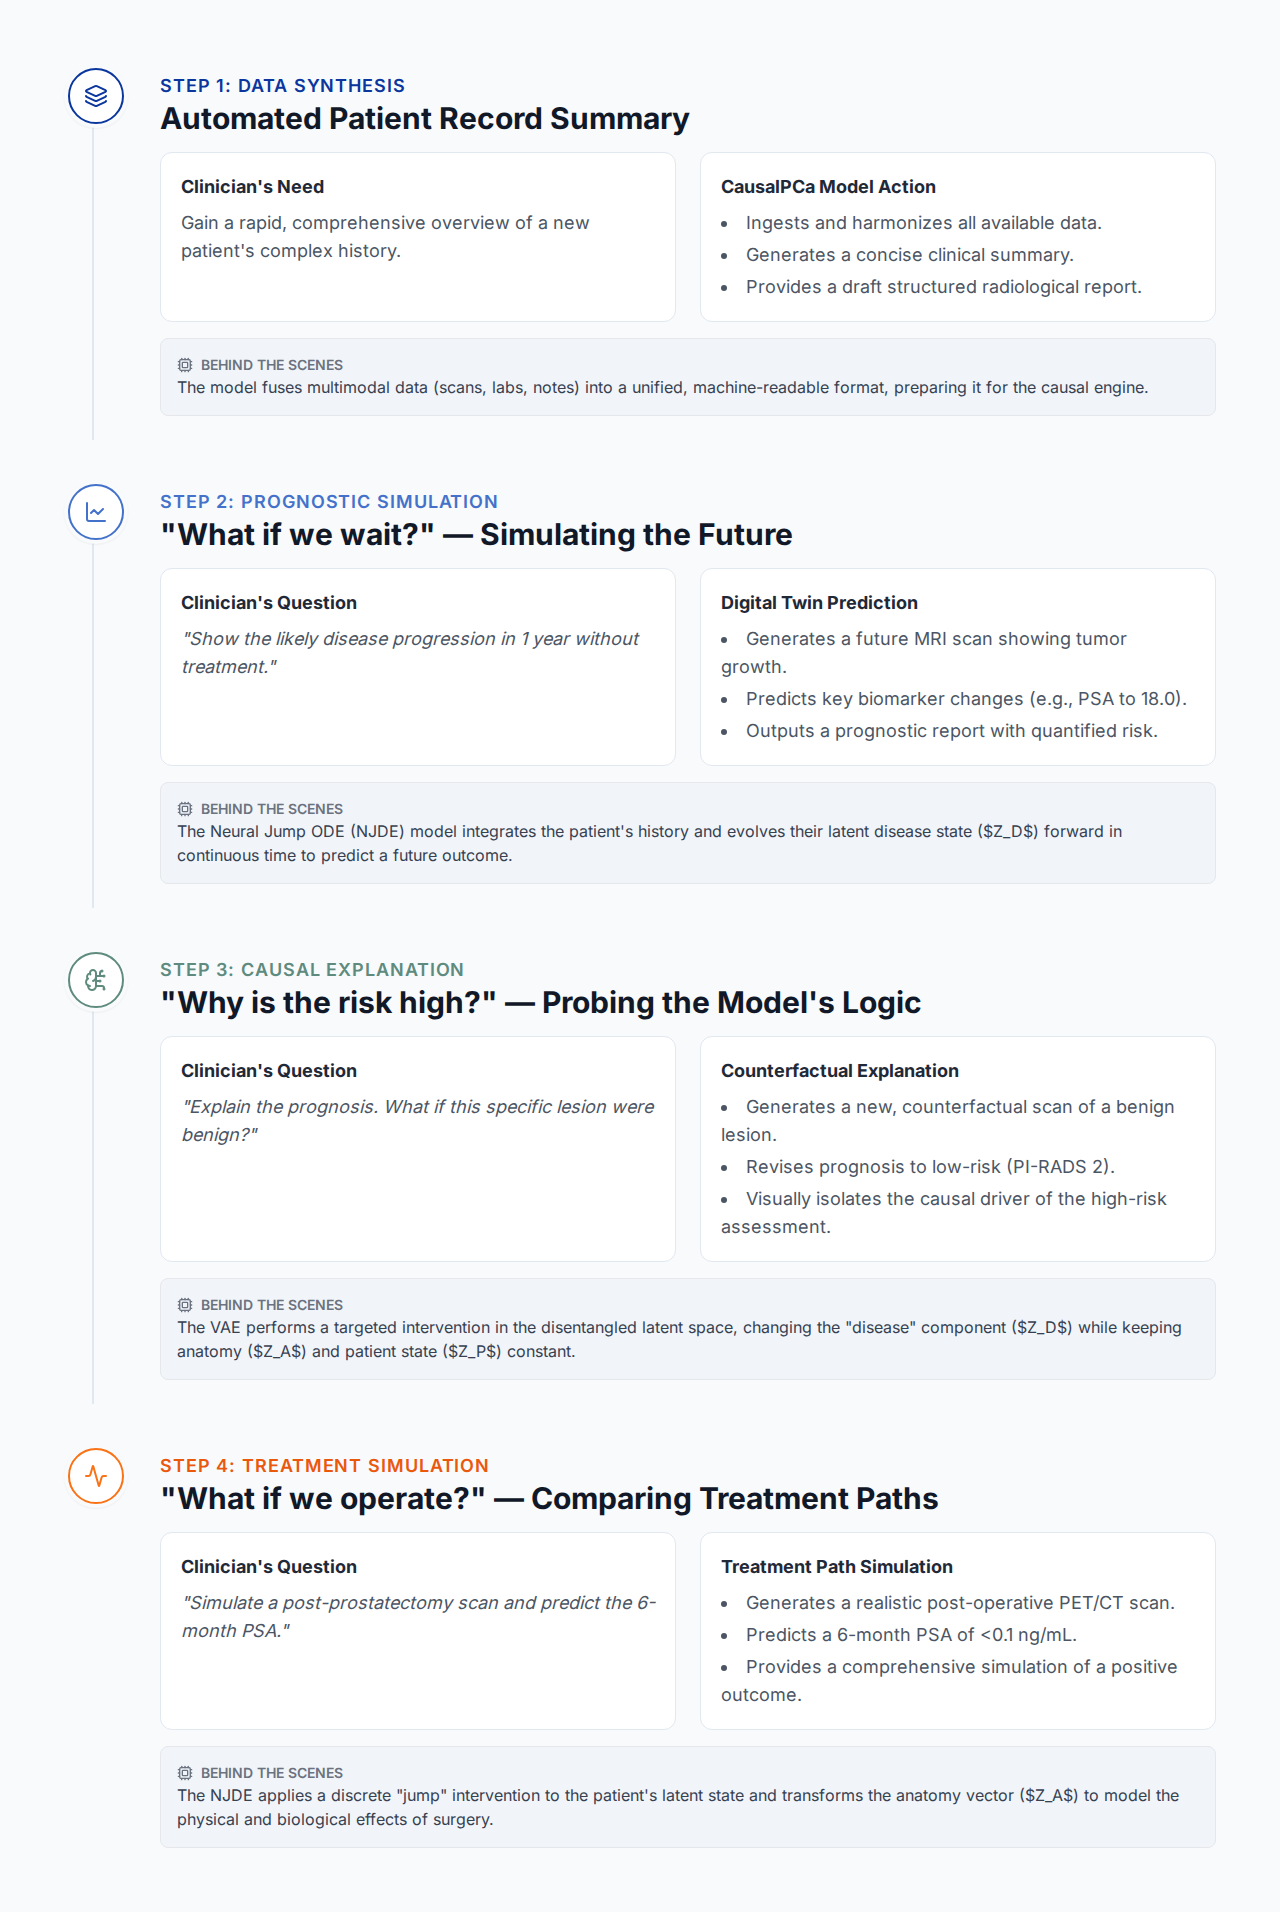
\includegraphics[width=1\textwidth]{wf.png}
    \caption{The Multidisciplinary Workflow of Prostate Cancer Diagnosis: A complex, iterative process requiring multimodal data fusion and expert collaboration.}
    \label{fig:workflow}
\end{figure}


\section{The Multidisciplinary Challenge of PCa Management and the Role of Automation}
The effective management of prostate cancer is an inherently complex and collaborative endeavor, demanding the integration of diverse, multimodal data and the expertise of numerous medical specialists. The entire process, from diagnosis to treatment planning and follow-up, creates a significant workload and contains points of subjectivity that are ripe for improvement through automation and Artificial Intelligence (AI) \cite{MohseniniaZamaniSiahkali2024, FerroCobelli2022}.

Radiologists and nuclear medicine physicians interpret a wide array of complex imaging studies, including mpMRI and PET/CT. Urologists and oncologists must then synthesize these imaging findings, pathology reports, clinical notes, and laboratory data like PSA levels to manage patient care. Finally, these specialists often convene in multidisciplinary tumor boards to collectively review all available information and formulate a consensus treatment plan based on established guidelines \cite{MohseniniaZamaniSiahkali2024, UnknownAuthor2017}.

This intricate, multi-step workflow is not only labor-intensive but also susceptible to variability at each stage. Artificial intelligence (AI) offers a powerful solution to these challenges. AI can automate tedious tasks, such as the extraction of quantitative image features, to reduce workload and improve consistency \cite{MohseniniaZamaniSiahkali2024, ChaddadTan2023}. By providing objective, reproducible data and streamlining workflows, AI has the potential to support the entire clinical team, ultimately enabling a more precise and personalized approach to prostate cancer care \cite{LaroseArchambault2024, BhattacharyaKhandwala2022}.Worflow is summarised on \ref{fig:workflow}


\section{The Challenge of Bias from Incomplete and Heterogeneous Data}
The development of generalizable AI models in oncology is profoundly challenged by biases that arise from incomplete and heterogeneous data. This is particularly true for a multi-center retrospective study such as this, where variability is inherent. These biases can compromise model integrity and lead to inequitable outcomes \cite{VenugopalGupta2023, CorreaShaan2022}.

A fundamental source of these challenges is that standard AI models, by default, treat all pixels and features in an image with equal importance. Without explicit guidance, they lack the intrinsic understanding to distinguish between clinically relevant pathology and irrelevant confounders such as scanner type, image noise, or incidental anatomical variations. This necessitates the integration of domain knowledge directly into the model's architecture to force it to ignore spurious correlations and focus only on the most diagnostically important information.

A critical issue is technical bias from data heterogeneity. Datasets compiled from multiple institutions using different scanners and protocols introduce systematic variations in image characteristics unrelated to the underlying biology \cite{SeoniShahini2024, HadjiiskiCha2023}. Models can inadvertently learn these site-specific signatures as "shortcuts," leading to excellent performance on internal data but poor generalization to new, unseen data \cite{LuoHuang2024, SouzaWinder2024}.

Equally problematic is bias from underrepresentation. If training data lacks sufficient examples of rare but aggressive histological subtypes or tumors in uncommon locations, the model may fail to learn their specific features. This leads to spectrum bias, where the model performs well on common presentations but fails on less frequent, yet clinically critical, cases \cite{Kocak2022, HattKrizsan2022}.

Finally, bias from missingness is a reality of retrospective data. In multi-modal studies, patients are often missing an entire imaging modality (patchwork learning) \cite{TerrailAyed2022}. Naive case deletion can introduce significant bias, as the reasons for missingness are often non-random and may correlate with disease characteristics, skewing the dataset \cite{Kocak2022, MartnezGarcaHernndezLemus2022}. The introduction of complex treatment data, such as from RLT, adds another layer of potential confounders. Minor, clinically insignificant variations in RLT protocols can become powerful confounding variables that an AI might learn as proxies for outcome, masking the true biological drivers of response \cite{PatellKurian2023, SadaghianiSheikhbahaei2022, GeorgeSamuel2023}.

\section{Limitations of Current Predictive Models and the Need for a Biologically Grounded Approach}
While the field of quantitative image analysis holds immense promise, its models are not yet universally proven to outperform classical clinical prediction models \cite{MolinBarry2024, FerroCobelli2022}. The process of extracting a large number of quantitative features from medical images, with the hypothesis that these features reflect underlying tumor biology \cite{MohseniniaZamaniSiahkali2024}, is hampered by significant methodological limitations, many of which are shared by other advanced computational models when applied to complex medical data.

\subsection{Data Scarcity, Dimensionality, and Standardization}
A primary challenge is the "curse of dimensionality," where the vast number of extracted quantitative features far exceeds the number of patients in a typical study. This creates a high risk of building models that are overfitted to the training data, capturing statistical noise rather than true biological signals, and severely limits their generalizability \cite{KendrickFrancis2021, GinsburgRsu2014}. Medical datasets, particularly those with high-quality 3D data like CT or PET, are scarce and costly to acquire, which further constrains model development \cite{AydinHilbert2024, Hanigutyt2024}. This issue is compounded by a lack of standardization in image acquisition and feature extraction methods, which makes it difficult to reproduce findings across different studies \cite{MolinBarry2024, MolinBarry2025}. The acquisition of multi-modality data is often incomplete due to clinical constraints, leading to missing data which is a significant hurdle for any predictive model \cite{KazerouniAghdam2022, LiLi2024}.

\subsection{Challenges in Disentangling Causal Factors}
Deep learning models are prone to learning shortcuts from spurious correlations in the data rather than true causal relationships \cite{AydinHilbert2024, FayCobos2023}. For example, a model might link disease prediction to irrelevant factors like scanner type instead of the underlying pathology \cite{FayCobos2023, VigneshwaranOhara2024}. Generative models, such as VAEs, attempt to learn the underlying data-generating factors, but their latent representations often remain entangled, meaning a single latent factor influences multiple output features, which hampers interpretation and control \cite{CetinStephens2022}. Enforcing disentanglement is notoriously difficult on complex medical data, where pathological features are inherently dependent on anatomical structures, and often comes at the cost of reduced image quality \cite{HuFalet2022, HavaeiMao2021}.

\subsection{Challenges in Modeling Longitudinal Data}
Modeling disease evolution over time introduces further complexity. Clinical data is typically sampled irregularly, which does not reflect the continuous nature of a patient's biological evolution \cite{SeedatImrie2022, Purohit2023}. Conventional time-series models often fail in this setting. The most significant challenge is handling time-dependent confounders—patient covariates (like health status) that are influenced by past treatments and in turn affect future treatments and outcomes \cite{Purohit2023, SeedatImrie2022}. Failure to account for this bias makes it difficult to estimate the true causal effect of interventions.

\subsection{The Path Forward: Biologically-Grounded Inductive Bias}
In several head-to-head comparisons for tasks like predicting survival in metastatic PCa, models based on established clinical variables have outperformed or performed equally to complex models based on quantitative image features \cite{MolinBarry2024, MolinBarry2025}. This suggests that simply increasing model complexity on high-dimensional data without sufficient domain knowledge is not a viable path forward. To overcome these limitations, the field must shift towards a more biologically grounded approach. This involves building models with strong inductive biases derived from established domain knowledge—namely, the pathophysiology of cancer and the influence of patient-specific characteristics. By developing methods to link imaging features to molecular data \cite{FerroCobelli2022, HuynhSwanson2024} and designing architectures that explicitly model known causal relationships, we can move beyond black-box data-mining and develop robust, interpretable tools for personalized medicine \cite{MolinBarry2025, GhezzoBezzi2022}.

\section{Study Population: Inclusion and Exclusion Criteria}
The study cohort will be established through a multi-center, retrospective collection of patient data, adhering to the following criteria:

\subsection{Inclusion Criteria}
\begin{enumerate}
    \item Patients with histopathologically confirmed (biopsy-proven) prostate adenocarcinoma.
    \item Availability of at least one baseline imaging study, either a multi-parametric MRI (mpMRI) or a PSMA-PET/CT scan.
\end{enumerate}

\subsection{Exclusion Criteria}
\begin{enumerate}
    \item Complete absence of any imaging data (MRI, PET/CT, or CT).
    \item Lack of recorded Prostate-Specific Antigen (PSA) values.
    \item Insufficient follow-up, defined as less than 6 months of clinical or biochemical data available after the initial imaging study.
    \item Presence of significant, irreconcilable conflicting information within the patient's medical records.
\end{enumerate}

\section{Proposed Framework for Comprehensive Data Collection and Bias Mitigation}
The successful development of advanced AI models is fundamentally dependent on collecting high-quality data in a standardized way. To address the challenges of incomplete and heterogeneous data, a standardized data collection pipeline is therefore a prerequisite for building robust and generalizable models \cite{SeoniShahini2024, StamoulouSpanakis2022}. The goal is to create a high-quality, longitudinal dataset that provides a solid foundation for advanced predictive modeling.

\subsection{Ethical Considerations and Data Security}
This study will be conducted in full compliance with ethical guidelines. Proper bioethical commission agreement will be acquired prior to the commencement of data collection. Data security and patient confidentiality are paramount. Data security will be preserved thanks to keeping data in XNAT, which allows for granularly controlled data access, ensuring that information is only accessible to authorized research personnel.

\subsection{Centralized Data Acquisition and Curation}
Our strategy begins with centralizing all patient data from every available time point into a secure repository like XNAT \cite{Marcus_2007}. All data undergoes a meticulous, non-destructive curation process where raw data is archived and all processing is performed on copies to ensure reproducibility \cite{KimKazmierski2025}. The following structured data will be collected and curated:

\subsubsection{Step 1: Initial Patient and Clinical Data}
This set of variables provides the foundational clinical context for each patient.
\begin{itemize}
    \item \textbf{Patient Demographics:} Age at the time of diagnosis.
    \item \textbf{Laboratory Data:} Prostate-Specific Antigen (PSA) level at diagnosis (ng/mL), along with timestamps for all laboratory results.
    \item \textbf{Histopathology:} Gleason Score from the prostate biopsy, categorized into ISUP Grade Groups.
    \item \textbf{Clinical Staging:} Clinical T-Stage (e.g., T2c, T3b). In cases where this is missing from records, it may be inferred from imaging.
    \item \textbf{Treatment Data:} Primary treatment method (e.g., surgery, radiation), with specific notation of whether Androgen Deprivation Therapy (ADT) was administered.
\end{itemize}

\subsubsection{Step 2: Imaging Data and Reports}
This includes all raw imaging files and their associated metadata and textual reports.
\begin{itemize}
    \item \textbf{Raw Imaging and Metadata:} Raw DICOM files from all modalities (PET, CT, MRI, SPECT), including post-therapy Lutetium scintigraphy, will be ingested. All scanner metadata and imaging timestamps will be preserved. Files undergo automated pseudonymization using libraries like \texttt{pydicom} \cite{JunqueroMartinezGirones2024, KondylakisKalokyri2023} and are converted to the NIFTI format (.nii.gz) for analysis.
    \item \textbf{Quantitative Imaging Features:} Key biomarkers will be extracted where applicable. For PSMA-PET/CT, this includes the Maximum Standardized Uptake Value (SUVmax) within the primary tumor.
    \item \textbf{Qualitative Imaging Features \& Reports:} Unstructured text from radiological reports will be collected. These reports will be automatically translated to English if necessary, then parsed using NLP methods to extract structured findings and map terminology to standardized vocabularies like SNOMED CT \cite{PesapaneTantrige2023}. Key extracted features include:
    \begin{itemize}
        \item For MRI: PI-RADS score for suspicious lesions.
        \item For PSMA-PET/CT: Presence/absence of Bone Metastases (OS\_Mx), Seminal Vesicle Invasion (SVI), Periprostatic/Extra-capsular Invasion, and Lymph Node Metastases (LNM) in specific anatomical regions (e.g., Common Iliac Bifurcation, Internal/External/Common Iliac). Also PSMA rads and promise description. 
    \end{itemize}
\end{itemize}

%https://g.co/gemini/share/01ead7d735d9
\begin{figure}[H]
        \centering
        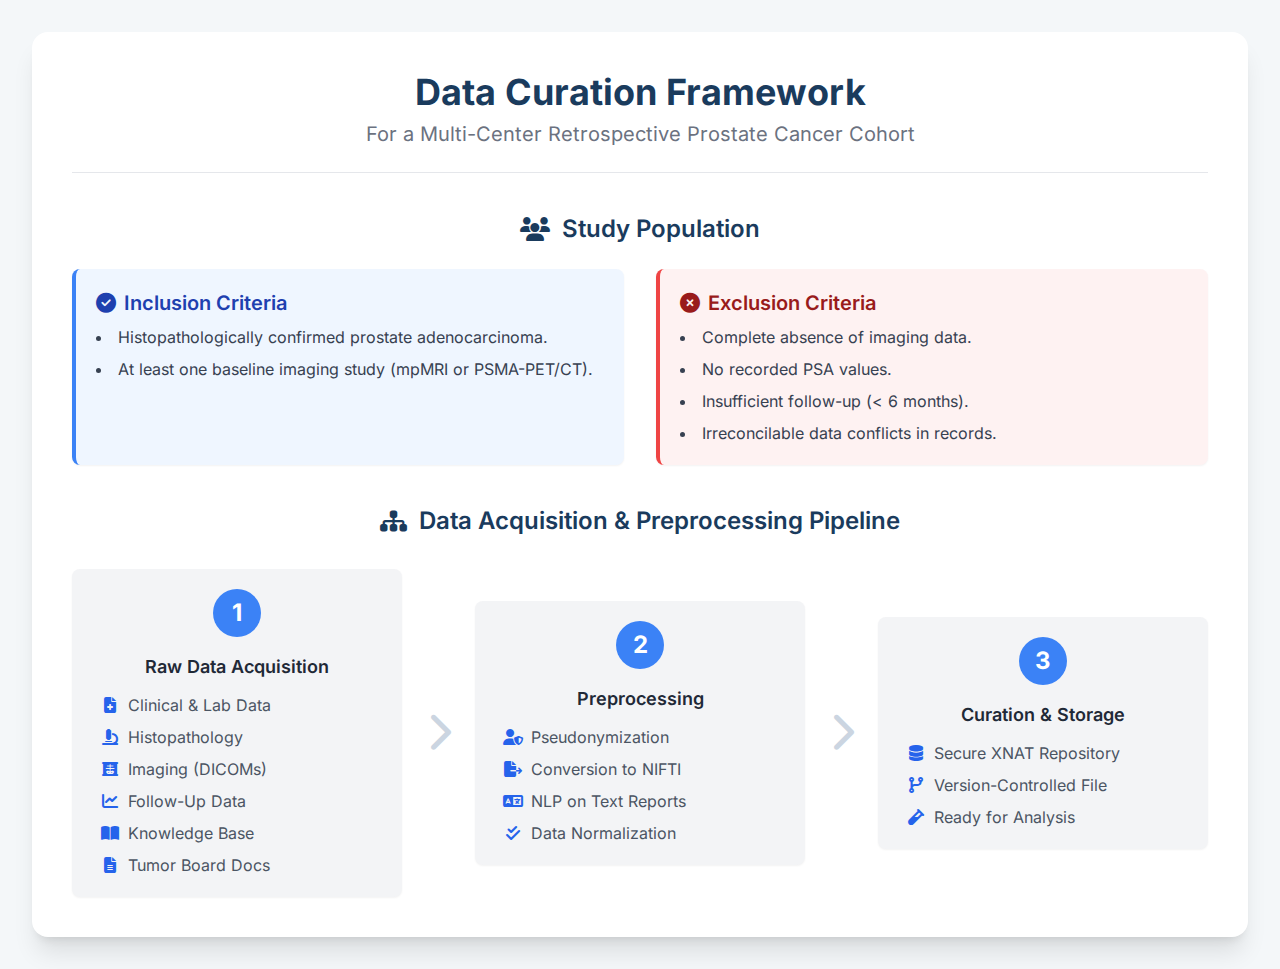
\includegraphics[width=\textwidth]{dc.png}
        \caption{An infographic summarizing the data acquisition, curation, and preprocessing framework for the study cohort. It details the inclusion and exclusion criteria for patient selection and outlines the multi-step pipeline for processing clinical, histopathological, and imaging data.}
        \label{fig:data_curation}
\end{figure}


\subsubsection{Step 3: Follow-up Data and Outcomes}
This longitudinal data is essential for modeling disease progression and validating prognostic endpoints.
\begin{itemize}
    \item \textbf{Follow-up Laboratory Data:} Serial PSA measurements taken after primary treatment, with corresponding timestamps.
    \item \textbf{Follow-up Imaging:} Results from any subsequent imaging studies used to confirm clinical progression.
    \item \textbf{Time to Follow-up:} The time interval between the initial imaging scan and the final assessment of the clinical outcome, which is critical for survival analysis.
\end{itemize}
All final curated tabular data is cleaned, normalized, and stored in a single version-controlled file.data collection ifs summaized on figure \ref{fig:data_curation}


\section{A Causal, Counterfactual Framework for Modeling Longitudinal Prostate Cancer Progression}


As described earlier the management of prostate cancer is a complex, data-intensive challenge. Clinicians must integrate diverse data streams—including advanced imaging like MRI, PSMA PET/CT, and Lutetium SPECT/CT, laboratory values like PSA, and unstructured clinical notes—to make critical decisions about a patient's care. A key difficulty is predicting an individual's disease trajectory over time from this sparse and irregularly sampled data. While modern deep learning models excel at pattern recognition, they often function as "black boxes," learning non-causal associations that can lead to erroneous and untrustworthy predictions. For instance, a model might associate a scanner artifact with disease severity, a shortcut that fails when presented with data from a new institution.

This section  outlines a novel framework designed to overcome these limitations by moving from spurious correlation to causal reasoning. We aim to build a robust, dynamic model of prostate cancer progression that learns the underlying causal mechanisms of the disease. By explicitly separating the signal (disease) from the noise (technical confounders), our model can generate clinically meaningful explanations. The core of our approach lies in the power of counterfactual reasoning—the ability to answer "what if" questions that mirror a clinician's own thought process and to simulate the outcomes of interventions like surgery. By generating visual counterfactuals (e.g., "What would this MRI look like if the lesion were benign?"), the model moves beyond simple prediction to become a transparent and collaborative decision support tool, essential for gaining clinical trust.







\section*{Conclusions}
In conclusion, this work addresses the profound challenge of managing prostate cancer by proposing a novel, biologically-grounded generative framework. We have detailed the limitations of current predictive models, which often fail to account for the complex, longitudinal, and multimodal nature of patient data, leading to a reliance on spurious correlations rather than true causal relationships.

Our proposed solution moves beyond conventional "black-box" approaches by introducing a multi-stage causal AI model. At its core, the framework leverages a meticulously standardized data pipeline to mitigate bias and a hierarchical variational autoencoder to disentangle the core components of the disease—separating patient anatomy and pathophysiology from technical confounders. The integration of a Neural Jump Differential Equation (NJDE) is a key innovation, enabling the model to learn the continuous dynamics of disease progression from sparse, real-world data while explicitly accounting for the discrete impact of clinical interventions like surgery or therapy.

The ultimate output of this framework is not merely a prediction, but a dynamic, explainable, and interactive tool for clinical decision support. By generating clinically plausible counterfactuals, the model can answer critical "what-if" questions, simulating disease trajectories and treatment outcomes. Furthermore, its ability to automatically generate structured, consistent reports has the potential to significantly reduce the clinical burden of documentation and enhance data quality for future research.

This research lays the groundwork for a new paradigm in predictive oncology, shifting the focus from simple pattern recognition to a deep, causal understanding of disease evolution. By creating a robust, trustworthy, and interpretable model of the individual patient's journey, this framework promises to enhance diagnostic accuracy, personalize treatment strategies, and ultimately improve outcomes for patients with prostate cancer.

\section*{Acknowledgments}
Artificial intelligence was used to aid in the creation of this manuscript. Specifically, the Gemini 2.5 Pro model was utilized for assistance with the literature review, for improving the style, grammar, and readability of the text, and for the collection and preparation of code for infographics.


\section{Model Architecture: A Multi-Stage Causal Framework}
To ensure stability and manage the complexity of multimodal data, the model is constructed using a sequential, multi-stage training framework. This approach decomposes the overall task into a series of manageable sub-problems, where each stage builds upon the foundations laid by the previous one.

\subsection{Stage 1: Training Foundational Supervisors}
The first stage involves training a suite of specialized "supervisor" models. These models act as expert guides, providing strong, accurate signals that will enforce a clinically valid structure on the more complex generative models in the subsequent stages. Each of these supervisors is based on established architectures and training paradigms for which practical implementation pathways have been demonstrated in the literature \cite{LeeByeon2025, GrisiKartasalo2025, RivailVogl2023, MehtaShui2023}.
\begin{itemize}
    \item \textbf{Ordinal Classifiers:} For clinical scores with an inherent order (e.g., PI-RADS, TNM stage), standard categorical classifiers using Cross-Entropy loss are suboptimal as they ignore the crucial ordering relationship (i.e., a higher grade implies a worse prognosis). To address this, we will train our classifiers using a more sophisticated \textbf{differential ordinal learning framework} \cite{LeeByeon2025}. This involves a multi-task approach where the model simultaneously learns to predict the specific class label and, critically, the degree of difference between pairs of samples, thus explicitly encoding the ordinal structure. The total loss function will be a hybrid, combining a standard categorical loss with a specialized differential ordinal loss (such as Negative Absolute Difference Log-likelihood), which is explicitly designed to handle ordered classes more effectively than conventional methods \cite{GrisiKartasalo2025}. These classifiers, built on Vision Transformer (ViT) backbones, will be trained for TNM Staging, PI-RADS (MRI), and PSMA-RADS/PROMISE (PSMA PET/CT).
    \item \textbf{Censored Survival Regressor:} To predict time to progression (TTP), we will train a survival model that properly handles right-censored data (e.g., patients with less than 6 months of follow-up who have not yet progressed). This will be achieved using a censored regression loss (e.g., Logistic Hazard or an Accelerated Failure Time log-likelihood loss) combined with a ranking loss regularizer (e.g., SurvRNC) to ensure correct risk ordering in the learned feature representation \cite{GaoLi2019, RivailVogl2023, ShahinZhao2023, SaeedRidzuan2024, ApellnizParras2024}.
    \item \textbf{Anatomical Segmentator:} A pre-trained TotalSegmentator model will be fine-tuned to generate gold-standard anatomical segmentations. A version will be adapted to operate directly on tensors, providing a differentiable anatomical loss for the VAE training.
    \item \textbf{Patient State Regressor (Age):} As age is a critical risk factor and also drives benign anatomical changes, we will train a dedicated regressor to predict patient age from imaging. This allows us to explicitly model and control for age-related effects, separating them from pathology \cite{PuglisiAlexander2025, ZhangHager2025}.
    \item \textbf{Technical Confounder Classifiers:} To isolate non-clinical sources of variation, we will train classifiers for: scanner type, PSMA/Lutetium dosage, and patient BMI.
\end{itemize}

\subsection{Stage 2: Per-Modality Causal Representation Learning}
For each imaging modality $m$, we train a separate hierarchical Variational Autoencoder (VAE), likely based on an efficient 3D Vision Transformer (ViT) or 3D CNN backbone, to learn a disentangled latent space, $Z_m$ \cite{KimOh2025, LeeByeon2025, FragemannArdizzone2022}. The VAE compresses a high-dimensional image $x_m$ into a low-dimensional summary (the latent space) and then reconstructs it \cite{HeSarwal2024, FriedrichFrisch2024}. The key innovation is that this latent space is partitioned into independent, semantically meaningful components:
$$ Z_m = Z_A \oplus Z_D \oplus Z_P \oplus Z_S $$
Here, $\oplus$ denotes concatenation, and the components represent \textbf{Anatomy} ($Z_A$), \textbf{Disease} ($Z_D$), \textbf{Patient State} (age-related changes, $Z_P$), and \textbf{Style/Shortcut} (technical artifacts, $Z_S$). This separation is enforced through a complex, multi-stage training process governed by a composite loss function that leverages the supervisors from Stage 1.

\subsubsection{Composite Loss Function and Staged Training}
The training is carefully staged to ensure stability and guide the VAE towards the correct solution. The total loss, $\mathcal{L}_{\text{total}}$, is a weighted sum of several components:
$$ \mathcal{L}_{\text{total}} = \mathcal{L}_{\text{VAE}} + \lambda_A \mathcal{L}_{\text{Anatomy}} + \lambda_D \mathcal{L}_{\text{Disease}} + \lambda_I \mathcal{L}_{\text{Disentangle}} $$
The core VAE loss, $\mathcal{L}_{\text{VAE}}$, consists of a reconstruction term and a Kullback-Leibler (KL) divergence term, $D_{KL}(q_{\phi}(Z|X)||p(Z))$, which regularizes the learned latent space. The training proceeds as follows:
\begin{enumerate}
    \item \textbf{Anatomy and Identity Pre-training (e.g., first 100 epochs):} The initial phase focuses on learning stable representations of anatomy and achieving high-fidelity reconstruction.
    \begin{itemize}
        \item \textbf{Anatomy Consistency ($\mathcal{L}_{\text{Anatomy}}$):} A synthetic image generated purely from the anatomy component ($Z_A$) is penalized if its segmentation (from the pre-trained TotalSegmentator) does not match the ground truth. Registration-guided consistency is also enforced, ensuring that elastic deformations applied to the input image result in corresponding deformations in the latent space \cite{LiChen2024}.
        \item \textbf{Healthy State Enforcement:} The image generated from $Z_A$ is passed to the disease classifiers from Stage 1, and the loss function penalizes any classification other than "healthy."
        \item \textbf{Identity Transformation:} To begin, the disease component ($Z_D$) is trained for identity transformation. The full reconstructed image (from $Z_A$ and $Z_D$) is supervised to match the original image's clinical labels (TNM, PI-RADS, etc.) using the Stage 1 classifiers. Standard reconstruction losses like L1 and multi-scale structural similarity are dominant here \cite{FerreiraLi2024, KhojasteSarakhsiHaghighi2024}.
    \end{itemize}
    \item \textbf{Generative and Disentanglement Training:} After the VAE has learned a stable anatomical basis, the training shifts to generative control and explicit disentanglement.
    \begin{itemize}
        \item \textbf{Generative Disease Control ($\mathcal{L}_{\text{Disease}}$):} The VAE is now tasked with a more complex goal. It receives a random target class (e.g., "PI-RADS 5" or "TNM Stage 3") and must modify the image generated from the anatomy component ($Z_A$) using the disease component ($Z_D$) such that the final image is correctly classified as the target class by the corresponding supervisor.
        \item \textbf{Explicit Disentanglement ($\mathcal{L}_{\text{Disentangle}}$):} The implicit regularization from the standard VAE's KL-divergence term is insufficient for robust disentanglement. Simply increasing its weight (as in a $\beta$-VAE) can degrade reconstruction quality by excessively penalizing the mutual information between the input and the latent space \cite{FragemannArdizzone2022, CetinStephens2022}. Our approach is more targeted. The KL-divergence term can be decomposed to isolate the \textbf{Total Correlation (TC)}, which specifically measures the statistical dependence among the individual latent dimensions \cite{FragemannArdizzone2022, AbbasiMonadjemi2018}. Our disentanglement loss, $\mathcal{L}_{\text{Disentangle}}$, will therefore heavily penalize the TC term, forcing the latent subspaces to become independent without sacrificing the information content needed for high-quality image generation. Furthermore, we will explicitly minimize the mutual information between specific subspaces that are causally independent, such as between the disease ($Z_D$) and style ($Z_S$) components, to ensure the learned disease representation is invariant to scanner-specific artifacts \cite{FayCobos2023}.
    \end{itemize}
\end{enumerate}

\subsection{Stage 3: Temporal Trajectory Modeling with Neural Jump ODEs}
This stage addresses the critical challenge of modeling disease evolution from sparse, multimodal, and irregularly-sampled clinical data. Our solution is a \textbf{Neural Jump Differential Equation (NJDE)} framework, which is uniquely suited for this task \cite{GwakSim2020}.

\subsubsection{Rationale and Latent State Formulation}
Neural Ordinary Differential Equations (NODEs) are powerful because they model system dynamics in continuous time, making them inherently robust to irregular sampling—a defining characteristic of clinical data \cite{GwakSim2020, JohnsonBulgarelli2023, BelogolovskyGreenberg2023}. However, their primary weakness is the extreme computational cost of applying them directly to high-dimensional data like 3D images \cite{WiewelBecher2018, DavisChoromanski2020}. Our approach strategically mitigates this by operating exclusively on the low-dimensional latent spaces learned in Stage 2. This is not just an efficiency gain; by training the NODE only on the disentangled \textbf{disease part of the latent space ($Z_D$)}, we focus the model on learning the dynamics of disease progression itself, making the learning task more tractable and clinically relevant \cite{AshmanSo2020, KberKalisch2023, LosadaTerranova2024}.

The input for the NJDE is a carefully constructed time series of latent state vectors. For each patient, we define a unified state vector $\mathbf{v}$ that has a fixed shape, representing a concatenation of all possible inputs. The process is as follows:
\begin{enumerate}
    \item \textbf{Unified State Vector Definition:} A canonical tensor shape is defined for a state vector $\mathbf{v}$, which includes dedicated slots for the disease latent code ($Z_D$) from each imaging modality (MRI, PET, SPECT) and for embeddings of all non-imaging data (PSA, clinical note embeddings, etc.).
    \item \textbf{Time-stamped Sparse Tensor Creation:} For each time point $t_i$ where a patient has data, a new state vector $\mathbf{v}(t_i)$ is created and initialized with zeros. The available data is then placed into its corresponding slot in the tensor. For example, at a time point with a PET scan and PSA value, only the $Z_{D_{\text{PET}}}$ and PSA embedding slots are filled, while all other slots (for MRI, notes, etc.) remain zero.
    \item \textbf{Anatomy Vector Storage:} The patient-specific anatomy vectors ($Z_A$) from each imaging study are not included in the dynamic state vector but are stored separately, indexed by time, for use in the final image reconstruction stage.
\end{enumerate}
This procedure yields a dataset of sparse, irregularly-sampled latent state vectors, providing a computationally efficient and robust representation of each patient's unique clinical history.

\subsubsection{NJDE Training and Dynamics}
The NJDE learns the rules of disease evolution by modeling two phenomena \cite{GwakSim2020}:
\begin{itemize}
    \item \textbf{Continuous Evolution (The NODE):} Between clinical events, the disease state evolves smoothly. This is modeled by a classic NODE that learns the underlying dynamics from the sparse state vectors \cite{BergHasenclever2018}.
    $$ \frac{d\mathbf{v}(t)}{dt} = f(\mathbf{v}(t), t; \psi) \quad \text{for } t \neq t_k $$
    \item \textbf{Discrete Jumps (The Interventions):} At the specific time $t_k$ of a clinical intervention (e.g., prostatectomy, initiation of hormonal therapy), the continuous evolution is interrupted by a discrete "jump." A separate neural network, $g$, models this instantaneous change to the state vector based on the type of intervention \cite{CuchieroLarsson2019, AbushaqraXue2022}.
    $$ \mathbf{v}^+ = g(\mathbf{v}(t_k), \text{intervention}_k; \phi) \quad \text{for } t = t_k $$
\end{itemize}
This hybrid approach, which explicitly separates the continuous disease course from the rapid, external impacts of clinical interventions, is critical for accurately modeling a patient's journey \cite{GwakSim2020}. The model is trained using a leave-one-out strategy for each patient's time series: given all but one time point, its goal is to predict the complete state vector for the held-out time point. To handle the pervasive missing data, we employ a \textbf{masked loss function}. The loss is calculated only by comparing the predicted values to the ground truth for those elements of the state vector that were actually available (non-zero) at the target time point. This forces the model to learn a probable evolution for every data type, even from a highly incomplete dataset.

\subsection{Stage 4: Generative Synthesis and Clinical Outputs}
The final stage translates the model's internal representations back into clinically useful outputs, including high-fidelity images and actionable, structured text.

\subsubsection{Image Generation and Refinement}
A final image for any time point (past, present, or future) and for any modality is generated by combining the appropriate anatomy vector ($Z_A$) with the disease vector ($Z_D$) predicted by the NJDE. An additional model is trained on the anatomy vectors to simulate post-prostatectomy changes. To ensure clinical realism, the generated VAE image is passed through a lightweight Diffusion Model that acts as a post-processor, adding high-frequency textural details and sharpness.

\subsubsection{Structured Report and Recommendation Generation}
A key output of our framework is the generation of structured reports, which are critical for enhancing clinical quality, standardization, and efficiency \cite{JorgHalfmann2023}. Structured reports are more complete, reduce errors, and provide data that is immediately usable for AI training and research \cite{SacoranskyKwan2024}. Our system will produce two types of structured text outputs using a Transformer-based decoder:
\begin{itemize}
    \item \textbf{Structured Radiological Reports:} For any imaging study (real or counterfactual), the decoder will take the corresponding anatomy ($Z_A$), disease ($Z_D$), and patient state ($Z_P$) latent vectors as input. It will generate a report that follows a predefined schema (e.g., a Pydantic model) composed primarily of closed questions and standardized fields. A section for supplementary free-text narrative will be included, but this part will be ignored in subsequent modeling steps to enhance system robustness. This unique link to the latent space allows the model to generate a descriptive report not just for an existing scan, but also for a counterfactual one (e.g., "Describe the MRI if the patient were 10 years older.").
    \item \textbf{Tumor Board Recommendations:} The NJDE, by modeling both continuous progression and discrete treatment \textit{jumps}, produces a comprehensive, dynamic model of the entire patient trajectory. A separate generative module will take this complete trajectory as input—synthesizing all available information across all time points. Based on this history and the model's prediction of the future disease course, it will generate a structured report with recommendations for further patient management, effectively simulating a data-driven tumor board consultation.
\end{itemize}

\section{Embedding Clinical Domain Knowledge: A Principled Approach}
A core strength of this framework is the systematic embedding of clinical domain knowledge, which acts as a strong inductive bias, guiding the model to learn representations that are not only accurate but also medically coherent.
\begin{itemize}
    \item \textbf{Respecting Ordinality in Clinical Scores:} We treat clinical scores like PI-RADS and TNM not as arbitrary categories but as ordinal scales. By using ordinal loss functions, the model learns that misclassifying a PI-RADS 2 as a 5 is a much graver error than misclassifying it as a 3.
    \item \textbf{Mimicking Clinical Reasoning via Disentanglement:} The separation of patient anatomy ($Z_A$) from disease ($Z_D$) mirrors how a radiologist thinks. A clinician first establishes the baseline anatomy and then identifies pathological deviations. By grounding the disease space ($Z_D$) with supervisors trained on clinical standards, we ensure the model's concept of "disease" is consistent with established diagnostic practice. This aligns with the inherently counterfactual nature of clinical diagnosis, where an expert might reason, "for this to be cancer, I would expect to see feature X."
    \item \textbf{Modeling Disease as a Continuous Process with Interventions:} Most AI models ignore the crucial temporal information in the intervals between scans. Our use of a Neural Jump ODE explicitly models disease progression as a continuous dynamic process that is punctuated by discrete, treatment-induced jumps. This allows the model to understand not only the significance of time but also the causal impact of interventions like surgery or therapy on the disease course.
\end{itemize}

\section{Illustrative Clinical Workflow}
Consider a clinician using the fully trained model for a new patient. The workflow demonstrates how the model provides actionable, explainable insights.
\begin{enumerate}
    \item \textbf{Automated Patient Summary:} The model ingests the patient's entire record and generates a concise summary, including a draft structured report for the latest scan.
    \item \textbf{Prognostic Inquiry:} The clinician asks, \textit{"Show prognosis in 1 year without treatment."}
    \begin{itemize}
        \item \textbf{Model Action:} The NJDE integrates the patient's history and solves its learned continuous differential equation forward in time to predict the disease state ($Z_D$) at $t+1$ year.
        \item \textbf{Model Output:} The model generates a future MRI showing tumor progression, a predicted PSA of 18.0 ng/mL, and an accompanying prognostic report.
    \end{itemize}
    \item \textbf{Explainable Reasoning Inquiry:} To understand a high-risk prediction, the clinician asks, \textit{"What if the primary lesion were benign?"}
    \begin{itemize}
        \item \textbf{Model Action:} The model performs a targeted intervention on the latent space, setting the disease component corresponding to the lesion to a "healthy" state while keeping all other factors constant.
        \item \textbf{Model Output:} It generates a new, counterfactual image where the lesion appears benign, along with a revised report: "PI-RADS 2."
    \end{itemize}
    \item \textbf{Treatment Planning Inquiry:} The clinician asks, \textit{"Show a post-prostatectomy PET scan and predict the PSA in 6 months."}
    \begin{itemize}
        \item \textbf{Model Action:} The model applies a "prostatectomy" intervention. This triggers a learned discrete \textbf{jump} in the NJDE to an immediate post-operative disease state. Simultaneously, a transformation is applied to the anatomy vector $Z_A$ to model the physical removal of the prostate. The NJDE then evolves this new state forward for 6 months.
        \item \textbf{Model Output:} It generates a realistic post-operative PET/CT scan and provides a predicted 6-month PSA value, offering a comprehensive simulation of the treatment outcome.
    \end{itemize}
\end{enumerate}

\section{Evaluation and Risk Management}
\subsection{Evaluation Metrics}
Model performance will be rigorously assessed using a comprehensive suite of metrics tailored to each sub-task.
\begin{itemize}
    \item \textbf{Classification:} Accuracy, Area Under the Curve (AUC), F1-Score, and Quadratic Weighted Kappa (for ordinal tasks).
    \item \textbf{Survival Regression:} Concordance Index (C-index) and Mean Absolute Error on censored data.
    \item \textbf{Image Generation:} Fréchet Inception Distance (FID), Structural Similarity Index (SSIM), and Learned Perceptual Image Patch Similarity (LPIPS) to measure realism and fidelity \cite{VigneshwaranOhara2024, Singla2022, LiShi2023, MoroSantinha2024, RossiLopez2024}.
    \item \textbf{Counterfactual Quality:} A comprehensive suite of metrics to assess axiomatic soundness (effectiveness, composition, reversibility) \cite{KomanduriWu2023, MonteiroRibeiro2023}, validity (success rate of flipping a classifier’s decision) \cite{SinglaEslami2021, Singla2022}, proximity (distance to the original) \cite{GuoDeng2024}, and realism (FID) \cite{VigneshwaranOhara2024, Singla2022}.
\end{itemize}

\subsubsection{Uncertainty Quantification for Downstream Tasks}
A significant advantage of our VAE-based architecture is its intrinsic ability to quantify uncertainty, a critical feature for high-stakes clinical decision-making. The probabilistic nature of the VAE encoder, which maps an input image to a distribution (mean $\mu$ and variance $\sigma^2$) rather than a single point, allows us to estimate the model's confidence in its predictions \cite{FriedrichFrisch2024, GautierBousse2024}. We will employ two complementary methods:
\begin{itemize}
    \item \textbf{Latent Space Sampling:} For a given input, we will draw multiple samples ($z_1, z_2, ..., z_N$) from its learned latent distribution using the reparameterization trick \cite{AbbasiMonadjemi2018}. Each sample will be passed to the downstream model (e.g., the NJDE or a classifier), yielding a distribution of output predictions. The variance of this output distribution will serve as a robust measure of the model's epistemic uncertainty (i.e., its confidence in its own learned representation) \cite{BustinMeyer2025}.
    \item \textbf{Direct Variance Utilization:} The variance vector $\sigma^2$ directly produced by the VAE encoder is itself an indicator of the model's uncertainty about its encoded features \cite{FriedrichFrisch2024}. We will concatenate this variance vector with the mean vector $\mu$ as a direct input to our downstream models. This explicitly informs the prediction models about the reliability of each feature in the latent representation, allowing the model to learn to depend more on high-confidence features.
\end{itemize}

\subsection{Clinical Plausibility and Workflow Integration Study}
Beyond quantitative metrics, a practical, clinician-in-the-loop study is essential to assess the model's real-world utility and trustworthiness.
\begin{itemize}
    \item \textbf{Assessing Counterfactual Plausibility and Usefulness:} To evaluate the quality of our generated explanations, we will conduct a human-grounded study with radiologists and oncologists. Clinicians will be presented with a series of cases, each including an original image and its corresponding model-generated counterfactual (e.g., an image of a tumorous prostate and its benign-looking counterfactual). They will score the counterfactuals on a Likert scale for:
    \begin{itemize}
        \item \textbf{Clinical Plausibility:} Does the generated image appear realistic and anatomically sound? \cite{GuoDeng2024, RossiLopez2024}
        \item \textbf{Usefulness for Explanation:} Does the visual difference between the original and counterfactual image provide a clear and understandable reason for the model's prediction? \cite{SinglaEslami2021, Singla2022}
        \item We will also quantitatively verify that the generated changes correspond to statistically significant differences in relevant clinical metrics (e.g., tumor volume, ADC values, PSMA uptake), confirming that the model has learned clinically relevant features \cite{SinglaEslami2021, Singla2022}.
    \end{itemize}
    \item \textbf{Measuring Workflow Improvement with Structured Reports:} To assess the impact of the automated reports, we will perform a comparative workflow study. A control group of clinicians will review patient cases using traditional free-text reports and standard image viewers. An experimental group will review the same cases using our system's auto-generated structured reports and prognostic visualizations. We will measure:
    \begin{itemize}
        \item \textbf{Efficiency:} Time taken to extract key information (e.g., TNM stage, PI-RADS score, presence of key findings) required for treatment planning \cite{UnknownAuthor2020}.
        \item \textbf{Accuracy and Concordance:} Inter-rater agreement and accuracy of the extracted information compared to an expert-defined ground truth \cite{UnknownAuthor2020}.
        \item \textbf{User Satisfaction:} Clinicians' perceived efficiency, clarity, and confidence in their decisions will be assessed using a standardized questionnaire (e.g., the System Usability Scale) \cite{SinglaEslami2021, Singla2022}.
    \end{itemize}
\end{itemize}

\subsection{Risk Analysis and Mitigation Strategies}
This is an ambitious project with significant technical challenges. We have identified the primary risks and our corresponding mitigation strategies.
\begin{itemize}
    \item \textbf{Risk 1: Training Instability and Data Scalability.}
    \item \textbf{Mitigation:} Our primary mitigation is the \textbf{sequential training framework}. By decomposing a single, intractable optimization problem into a series of manageable sub-problems, we enhance stability and improve data efficiency.
    
    \item \textbf{Risk 2: Generalizability and Overfitting to Spurious Correlations.}
    \item \textbf{Mitigation:} We will embed strong \textbf{domain knowledge as inductive biases}. The architectural constraints, such as enforcing anatomy consistency and explicitly disentangling clinical content from technical artifacts via the composite loss function, guide the model to learn true causal factors.
    
    \item \textbf{Risk 3: Performance with Incomplete and "Messy" Retrospective Data.}
    \item \textbf{Mitigation:} Multi-center retrospective data is notoriously heterogeneous and incomplete. Our framework directly confronts this through its \textbf{Neural Jump ODE architecture}, which is inherently designed to handle sparse, irregularly sampled data. Furthermore, the use of a \textbf{masked loss function} during NJDE training is a key technique to learn from the available data without being penalized for the pervasive missingness.

    \item \textbf{Risk 4: Reliance on Natural Language Processing (NLP).}
    \item \textbf{Mitigation:} While powerful, NLP models are not infallible. We mitigate the risk of errors by focusing the model on extracting relatively simple, standardized scoring systems (like PI-RADS) and binary findings, which are less prone to error than complex narratives. Using standardized terminologies further reduces ambiguity.

    \item \textbf{Risk 5: Selection Bias.}
    \item \textbf{Mitigation:} The inclusion criteria may inadvertently select for patients from more advanced centers. While this bias is inherent to the research question, the \textbf{multi-center nature of the data collection} is the best possible mitigation, as it will capture variations in practice and patient populations across different institutions.
    
    \item \textbf{Risk 6: Clinical Trustworthiness and the "Black Box" Problem.}
    \item \textbf{Mitigation:} Our primary strategy for building trust is \textbf{explainability through counterfactuals}. This mechanism allows clinicians to probe the model's reasoning by asking "what-if" questions, transforming it from an opaque oracle into a verifiable partner.
\end{itemize}
\bibliographystyle{unsrt}

\bibliography{bibl}

\end{document}


Ethical practice and ai act links from pdf
Cancer image europe platform encouraged to be used 
Uncertainty  can be done via sampling encoders multiple times and verifying weather the outcome would change ... or how many times it would be the same .. 
Add more about sources of data that we have initiatives etc. 
Frame lutetiun psma as innovative treatment ... 
Dataset size geographical variability ... 